\label{System Architecture}

In this chapter we shall discuss how data is processed and transformed in order to obtain 
the information required by the graphical library. We shall highlight the main system components 
which perform modifications on the graph data, starting with the Tokenizer which reads the input 
files and ending with the Eclipse Draw-2D API. The system components and their connection is presented 
in figure \ref{sysarch}.

\section{Input file processor}

Input graphs are initially described in a source text file in a pseudo programming language (discussed in 
Chapter \ref{implem}). These files must be analyzed in order to extract the information 
regarding edges and vertexes. This is achieved by using a parser.

This parser splits the input file into a list of tokens and then traverses this list, searching for certain 
keywords and constructs, as specified by the grammar. When a keyword describing a graph element is encountered, 
subsequent tokens are extracted until the expression for that graph element is completed. Using this expression 
and the information it contains, a corresponding vertex or edge object is created.

After the parser is finished extracting the data from the input file, it aggregates the vertexes and 
edges and constructs an object representing the graph. This object shall be the main container 
of information from now on. It is shared by the other components of the system, but all modifications are perfromed 
iteratively, never concurrently.

\section{Planarity tester}

After the graph container object is created, the first computational unit notified is the planarity tester. 
From the data which is provided by the graph container, the tester utilizes at first only the number of edges 
and vertices to apply the theorems mentioned in the Algorithm Design \ref{Algorithm Design} chapter. Should it fail 
to prove that the graph is not planar, the complete information regarding vertices and edges is extracted 
in order to apply the PQ-tree algorithm.

This unit does not modify the graph data in any way. Its result is stored internally and is accessed by the 
drawing library, which will display it as a relevant message for the user. Once the result has been stored, 
the layout processor is notified that it can access and perform operations on the container object.

\section{Layout processor}

This is the first unit which performs persistent modifications on the graph data. Its purpose is to determine 
the final coordinates for each node on the canvas, and mark the nodes as pinned, ensuring that no operation may 
modify their coordinates as a side-effect. Information about edges is also necessary, but only as an indication 
for the relationship between nodes.

Initially, the layout processor shall decide, based on the number of nodes, whether a grid layout or the genetic 
layout is more efficient. Generally, if the number of nodes is below a certain threshold, i.e. the algorithm is 
presented with a simple graph, it shall be layed out as a grid, otherwise the custom set of rules is applied. 
Next, the chosen algorithm is applied and the modifications are stored by the graph container object. A notification 
is then given to the connection router, so that it may begin the operating on the edges.

\section{Connection router}

The last step which must be performed before the graph is ready to be displayed is to compute the sets of points which compose 
the paths between nodes. The router is responsible with performing this operation.

The connection router analyses the existing edges in the graph container and builds corresponding orthogonal connectors.
This is a three-step operation:

\begin{itemize}

\item First, all nodes are connected directly using the shortest path method. All connections which are represented by 
vertical or horizontal lines that do not cross any other element are kept.

\item Second, those connections which did not match the criteria from step one are corrected (they are deviated to avoid 
obstacles). Also, connections which were not orthogonal before are orthogonalized.

\item Finally, a performance optimization is performed on connections. Redundant points are removed from paths (for example 
a segment which contains three points shall have the middle one removed) and paths which can be shortened without breaking 
the routing rules are modified accordingly.

\end{itemize}

Once this step is done, the graph container object holds all the data necessary for the drawing. This object shall be passed on 
to the drawing unit which utilizes the Eclipse draw-2D API.

\begin{figure}[ht] \centering
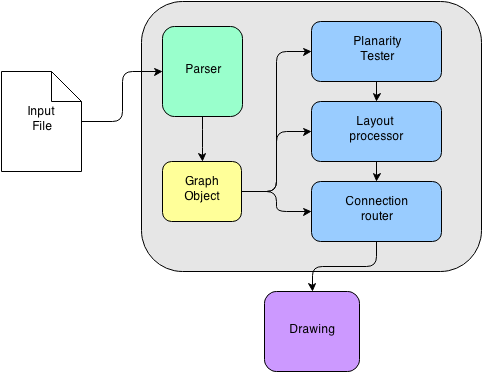
\includegraphics[width=0.65\textwidth]{img/systemarch/systemworkflow.png}
\caption{Diagram of the system workflow \label{sysarch}} \end{figure}
